% (The MIT License)
%
% Copyright (c) 2023 Yegor Bugayenko
%
% Permission is hereby granted, free of charge, to any person obtaining a copy
% of this software and associated documentation files (the 'Software'), to deal
% in the Software without restriction, including without limitation the rights
% to use, copy, modify, merge, publish, distribute, sublicense, and/or sell
% copies of the Software, and to permit persons to whom the Software is
% furnished to do so, subject to the following conditions:
%
% The above copyright notice and this permission notice shall be included in all
% copies or substantial portions of the Software.
%
% THE SOFTWARE IS PROVIDED 'AS IS', WITHOUT WARRANTY OF ANY KIND, EXPRESS OR
% IMPLIED, INCLUDING BUT NOT LIMITED TO THE WARRANTIES OF MERCHANTABILITY,
% FITNESS FOR A PARTICULAR PURPOSE AND NONINFRINGEMENT. IN NO EVENT SHALL THE
% AUTHORS OR COPYRIGHT HOLDERS BE LIABLE FOR ANY CLAIM, DAMAGES OR OTHER
% LIABILITY, WHETHER IN AN ACTION OF CONTRACT, TORT OR OTHERWISE, ARISING FROM,
% OUT OF OR IN CONNECTION WITH THE SOFTWARE OR THE USE OR OTHER DEALINGS IN THE
% SOFTWARE.

\documentclass{article}
\usepackage{../pmba}
\newcommand*\thetitle{Risk Management}
\begin{document}

\plush{\pmbaTitlePage{8}}

% reserves: management reserve too, contingency reserve

\plush{
\pptBanner{Management \st{Triangle} Rectangle}\par
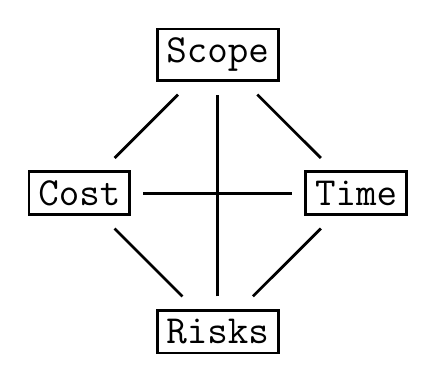
\begin{tikzpicture}[node distance=5em,
  every path/.style={draw=black, line width=.1em},
  every node/.style={font={\Large\ttfamily}, draw=black, rectangle, outer sep=.5em}]
\node[draw=none] (center) {};
\node[above of=center] (scope) {Scope};
\node[below of=center] (risks) {Risks};
\node[right of=center] (time) {Time};
\node[left of=center] (cost) {Cost};
\path (scope) -- (time);
\path (time) -- (cost);
\path (cost) -- (scope);
\path (risks) -- (time);
\path (risks) -- (cost);
\path (risks) -- (scope);
\end{tikzpicture}
}

\plush{
  \pptBanner{Read this:}
}

\end{document}
